% !TeX root = ../main_problemset.tex
\documentclass[../main_problemset.tex]{subfiles} % Inherits definitions from parent .tex file.

% Per-problem variable definitions
\newcommand{\problemName}{C. Sirkus Keliling}
\newcommand{\problemTL}{2 s}
\newcommand{\problemML}{256 MB}

\begin{document}

\begin{center}
    \section*{\problemName}
    \addcontentsline{toc}{section}{\problemName} % for pdf indexing
    
    \begin{tabular}{rl}
    Batasan waktu : & \problemTL \\
    Batasan memori : & \problemML
    \end{tabular}
\end{center}

\subsection*{Deskripsi}
\addcontentsline{toc}{subsection}{Deskripsi} % for pdf indexing

Terdapat N kota di Negeri Asgem, yang dinomori dari 1 hingga N. Masyarakat Asgem menyenangi sirkus. Terdapat satu tim sirkus lokal pada setiap kota. Biaya pertahun untuk menggaji tim sirkus lokal pada kota ke-i adalah S[i].

Negeri Astik menawarkan tim-tim sirkus keliling untuk beroperasi di Negeri Asgem. Setiap tim sirkus keliling memiliki rute tertentu yang harus memenuhi seluruh syarat di bawah ini:

\begin{itemize}
	\item Melalui 2 hingga N kota. Misalkan X adalah banyaknya kota yang dilalui oleh rute tersebut.
	\item Rute tersebut sirkular: secara berurutan, mulai dari kota K[1], kemudian menempuh sebuah ruas jalan menuju kota K[2], ..., kemudian menempuh sebuah ruas jalan menuju kota K[X], kemudian menempuh sebuah ruas jalan menuju kota K[1], dan seterusnya.
	\item \{K[1], K[2], ..., K[X]\} adalah kota-kota yang berbeda-beda.
\end{itemize}

Juga, agar masyarakat tidak bosan, setiap kota hanya boleh dilalui oleh paling banyak satu rute tim sirkus keliling.

Terdapat M ruas jalan \textbf{satu arah} di Negeri Asgem. Ruas jalan ke-i menghubungkan kota U[i] menuju kota V[i]. Untuk melewati ruas jalan tersebut, sebuah tim sirkus keliling akan dibebani ongkos tahunan sebesar W[i].

Pak Chanek, presiden Asgem, ingin melakukan penghematan anggaran tahunan pertunjukan sirkus. Oleh karena itu, ia berencana untuk merekrut nol atau lebih tim sirkus keliling, kemudian menghentikan operasi tim-tim sirkus lokal pada seluruh kota yang dilalui oleh rute-rute tim sirkus keliling tersebut. Anggaran tahunan pertunjukan sirkus akan menjadi total dari:

\begin{itemize}
	\item jumlah gaji seluruh tim sirkus lokal yang masih beroperasi, dan
	\item jumlah seluruh ongkos ruas jalan yang dilewati oleh seluruh rute tim sirkus keliling.
\end{itemize}

Bantulah Pak Chanek untuk meminimumkan anggaran tahunan pertunjukan sirkus, serta menentukan banyaknya tim sirkus keliling yang direkrut dan rute masing-masing tim sirkus keliling untuk mencapai anggaran minimum tersebut.

\subsection*{Format Masukan}
\addcontentsline{toc}{subsection}{Format Masukan} % for pdf indexing

Baris pertama berisi sebuah bilangan bulat T yang menyatakan banyaknya kasus uji. Baris-baris berikutnya berisi T kasus uji, yang masing-masing diberikan dalam format berikut ini:

\begin{lcverbatim}
N M
S[1] S[2] .. S[N]
U[1] V[1] W[1]
U[2] V[2] W[2]
.
.
U[M] V[M] W[M]
\end{lcverbatim}

\pagebreak
\subsection*{Format Keluaran}
\addcontentsline{toc}{subsection}{Format Keluaran} % for pdf indexing

Untuk setiap kasus uji, keluarkan jawaban dalam format berikut ini:

\begin{lcverbatim}
C R
X[1] K[1][1] K[1][2] .. K[1][X[1]]
X[2] K[2][1] K[2][2] .. K[2][X[2]]
.
.
X[R] K[R][1] K[R][2] .. K[R][X[R]]
\end{lcverbatim}

\vspace{.4cm}

\begin{minipage}[t]{0.5\textwidth}
\subsection*{Contoh Masukan}
\addcontentsline{toc}{subsection}{Contoh Masukan} % for pdf indexing

\begin{lcverbatim}
4
2 2
9 10
1 2 3
2 1 4
3 6
2 2 2
1 2 1
2 3 1
3 1 1
2 1 1
3 2 1
1 3 1
2 2
1 2
1 2 3
2 1 4
4 4
2 2 2 2
1 2 1
2 1 1
3 4 1
4 3 1
\end{lcverbatim}
\end{minipage}
\begin{minipage}[t]{0.5\textwidth}
\subsection*{(Salah Satu) Contoh Keluaran}
\addcontentsline{toc}{subsection}{Contoh Keluaran} % for pdf indexing

\begin{lcverbatim}
7 1
2 1 2
3 1
3 1 2 3
3 0
4 2
2 3 4
2 2 1
\end{lcverbatim}
\end{minipage}

\subsection*{Penjelasan}
\addcontentsline{toc}{subsection}{Penjelasan} % for pdf indexing

Untuk contoh pertama, anggaran sebesar 7 satuan adalah anggaran minimum yang mungkin dicapai. Berikut adalah ilustrasi penentuan sirkus yang sesuai dengan contoh keluaran (warna hijau menandakan sirkus yang ditentukan dalam anggaran minimum).

\begin{figure}[H]
	\centering
	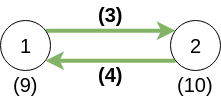
\includegraphics[width=120px]{bis-ddak/asset/Sample_1_OK}
\end{figure}

Perhatikan bahwa terdapat penganggaran yang tidak optimal yaitu jika kedua kota menggunakan sirkus lokal yang membutuhkan anggaran sebesar 19 satuan, seperti pada ilustrasi berikut.

\begin{figure}[H]
	\centering
	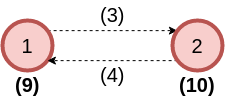
\includegraphics[width=120px]{bis-ddak/asset/Sample_1_NOT_OK}
\end{figure}

Untuk contoh kedua, anggaran sebesar 3 satuan adalah anggaran minimum yang mungkin dicapai. Terdapat tepat dua penentuan sirkus yang menghasilkan anggaran minimum, yaitu sesuai dengan dua ilustrasi berikut.

\vspace{-0.8cm}
\begin{minipage}[t]{0.5\textwidth}
\begin{figure}[H]
	\centering
	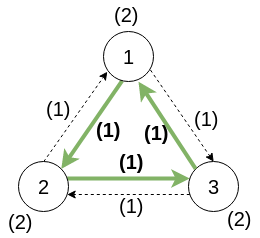
\includegraphics[width=120px]{bis-ddak/asset/Sample_2_OK_1}
\end{figure}
\end{minipage}
\begin{minipage}[t]{0.5\textwidth}
\begin{figure}[H]
	\centering
	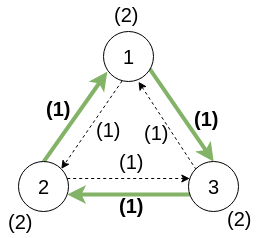
\includegraphics[width=120px]{bis-ddak/asset/Sample_2_OK_2}
\end{figure}
\end{minipage}
\vspace{0.1cm}

Berikut adalah contoh penentuan sirkus yang tidak optimal.

\begin{figure}[H]
	\centering
	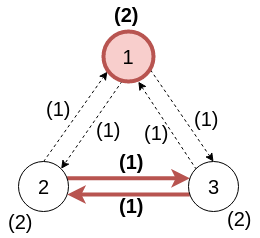
\includegraphics[width=120px]{bis-ddak/asset/Sample_2_NOT_OK}
\end{figure}

Untuk contoh ketiga, anggaran sebesar 3 satuan adalah anggaran minimum yang mungkin dicapai yaitu dengan tetap menggunakan sirkus lokal dari kedua kota.

\begin{figure}[H]
	\centering
	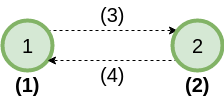
\includegraphics[width=120px]{bis-ddak/asset/Sample_3_OK}
\end{figure}

Untuk contoh keempat, anggaran sebesar 4 satuan adalah anggaran minimum yang mungkin dicapai, yaitu dengan menggunakan sirkus keliling untuk pasangan kota 1 dan 2 serta pasangan kota 3 dan 4.

\begin{figure}[H]
	\centering
	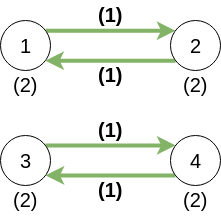
\includegraphics[width=120px]{bis-ddak/asset/Sample_4_OK}
\end{figure}

\subsection*{Batasan}
\addcontentsline{toc}{subsection}{Batasan} % for pdf indexing

\begin{minipage}[t]{0.47\textwidth}
	
Batasan yang berlaku untuk versi mudah dan versi sulit:

\begin{itemize}
	\item 1 $ \leq $ T $ \leq $ 5
	\item 1 $ \leq $ M $ \leq $ N $ \times $ (N - 1)
	\item 1 $ \le $ S[i], W[i] $ \le $ 8.000.000
	\item 1 $ \le $ U[i], V[i] $ \le $ N
	\item U[i] $ \neq $ V[i]
	\item (U[i], V[i]) $ \neq $ (U[j], V[j]) untuk i $ \neq $ j
\end{itemize}
\end{minipage}
\begin{minipage}[t]{0.06\textwidth}
	\hfill
\end{minipage}
\begin{minipage}[t]{0.47\textwidth}
	Batasan khusus versi mudah:
	\begin{itemize}
		\item 1 $ \le $ N $ \le $ 12
	\end{itemize}
	
	\vspace{.2cm}
	
	Batasan khusus versi sulit:
	\begin{itemize}
		\item 1 $ \le $ N $ \le $ 250
	\end{itemize}
\end{minipage}

\end{document}
